\documentclass[12pt,a4paper]{article}
\usepackage[utf8x]{inputenc}
\usepackage{ucs}
\usepackage[spanish]{babel}
\usepackage{amsmath}
\usepackage{amsfonts}
\usepackage{amssymb}
\usepackage{makeidx}
\usepackage{graphicx}
\usepackage[hidelinks]{hyperref}
\usepackage[left=2cm,right=2cm,top=2cm,bottom=2cm]{geometry}
\author{Reyes Alvarez Ulises Isaac\\4.B    Ing. Mecatrónica\\Mtro. Carlos Enrique Morán Garabito\\Sistemas electrónicos de interfaz\\Ago - Dic 2019}
\title{Amplificadores Clase A}
\begin{document}
\maketitle
\begin{figure}[hbtp]
\centering

\includegraphics[scale=1.7]{Circuitos/Universidad.png}
\end{figure}

\newpage
\section*{Amplificadores Clase A}
Son aquellos amplificador cuyas etapas de potencia consumen corrientes altas y continuas de su fuente de alimentación, independientemente de si existe señal de audio o no.

\section{Características}
Esta amplificación presenta el inconveniente de generar una fuerte y constante emisión de calor. No obstante, los transistores de salida están siempre a una temperatura fija y sin alteraciones. En general, se afirma que esta clase de amplificación es frecuente en circuitos de audio y en los equipos domésticos de gama alta, ya que proporcionan una calidad de sonido potente y de muy buena calidad.\\
Los amplificador de clase A a menudo consisten en un transistor de salida conectado al positivo de la fuente de alimentación y un transistor de corriente constante conectado de la salida al negativo de la fuente de alimentación. La señal del transistor de salida modula tanto el voltaje como la corriente de salida. Cuando no hay señal de entrada, la corriente de polarización constante fluye directamente del positivo de la fuente de alimentación al negativo, resultando que no hay corriente de salida, se gasta mucha corriente. Algunos amplificador de clase A más sofisticados tienen dos transistores de salida en configuración push-pull.

\section{Funcionamiento}
En este caso la máxima señal de salida se obtendrá cuando el punto estático coincida con el centro de la recta de carga, consiguiendo, por tanto, la máxima potencia de salida. Se pueden presentar en dos casos en cuanto a la conexión de la carga, estos es, que la carga, a la que hay que aplicar la potencia, sea externa al circuito o, que ésta sea la propia carga del transistor. A pesar de su escasa utilización, cuando se emplean suele coincidir con está última disposición.\\
Ambos casos se han de ver bajo el punto de vista de las rectas de carga: en el primero, son distintas para CC y CA; y en el segundo caso, coinciden para cargas resistivas.\\
\begin{figure}[hbtp]
\centering
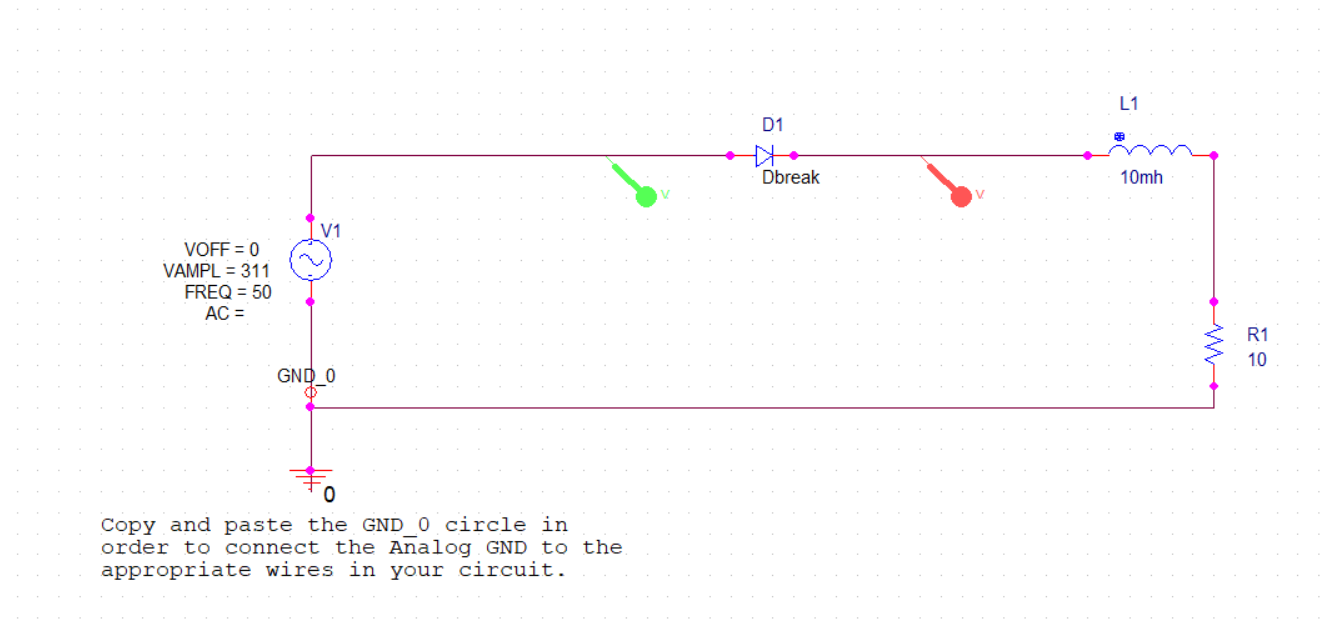
\includegraphics[scale=1]{Circuitos/1.png}
\caption{Amplificador Clase A}
\end{figure}
\newpage
Nótese que es un par de Darlington para aprovechar su elevada ganancia de corriente. En todo caso, la ganancia total obtenida será la corriente, manteniéndose la tensión de salida prácticamente al mismo nivel de entrada y cumpliendo, por tanto, las características de los amplificadores de potencia. La máxima ganancia se obtendrá cuando el punto Q se situé en el centro de la recta de la carga. 
\begin{figure}[hbtp]
\centering
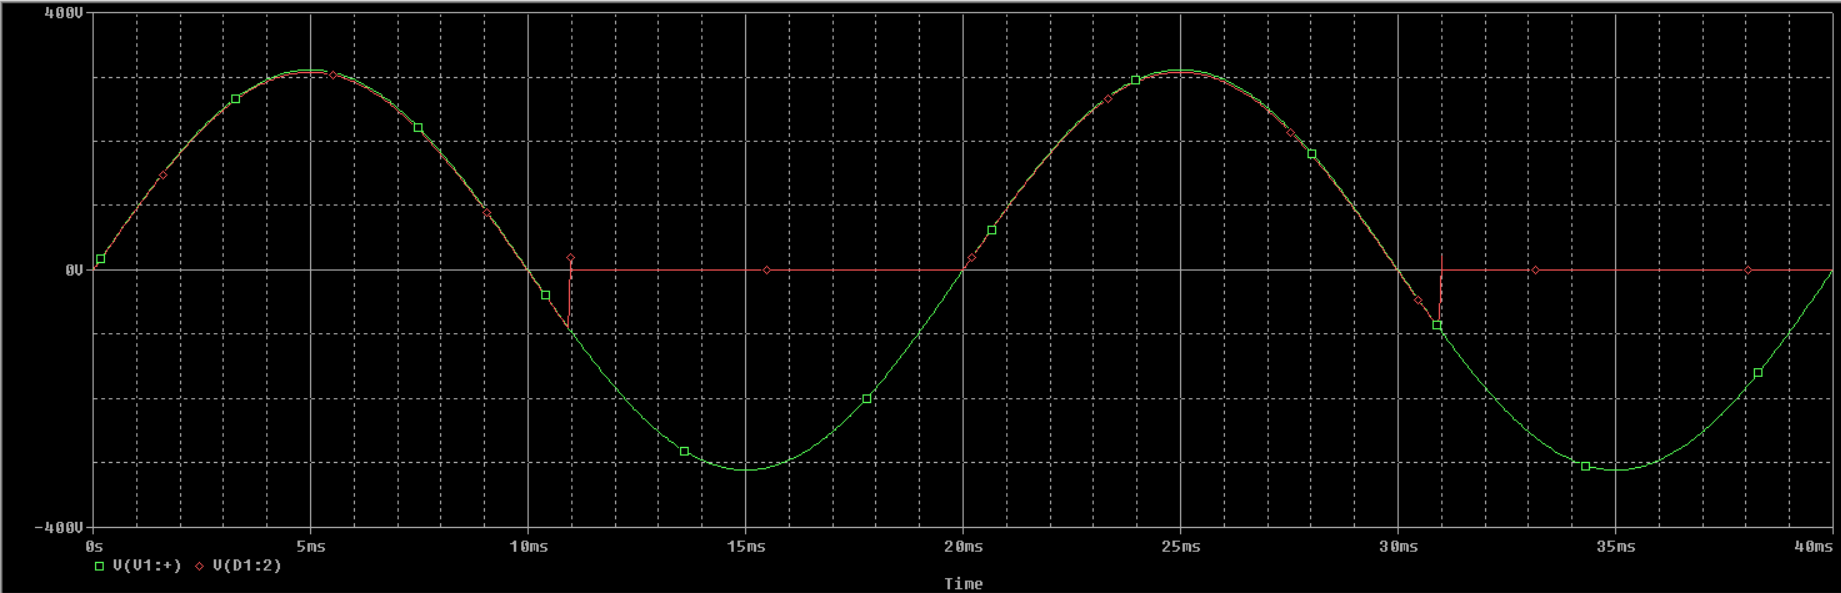
\includegraphics[scale=1]{Circuitos/2.png}
\caption{Recta de la carga y punto Q en clase A}
\end{figure}

\section{Eficiencia}
\begin{figure}[hbtp]
\centering
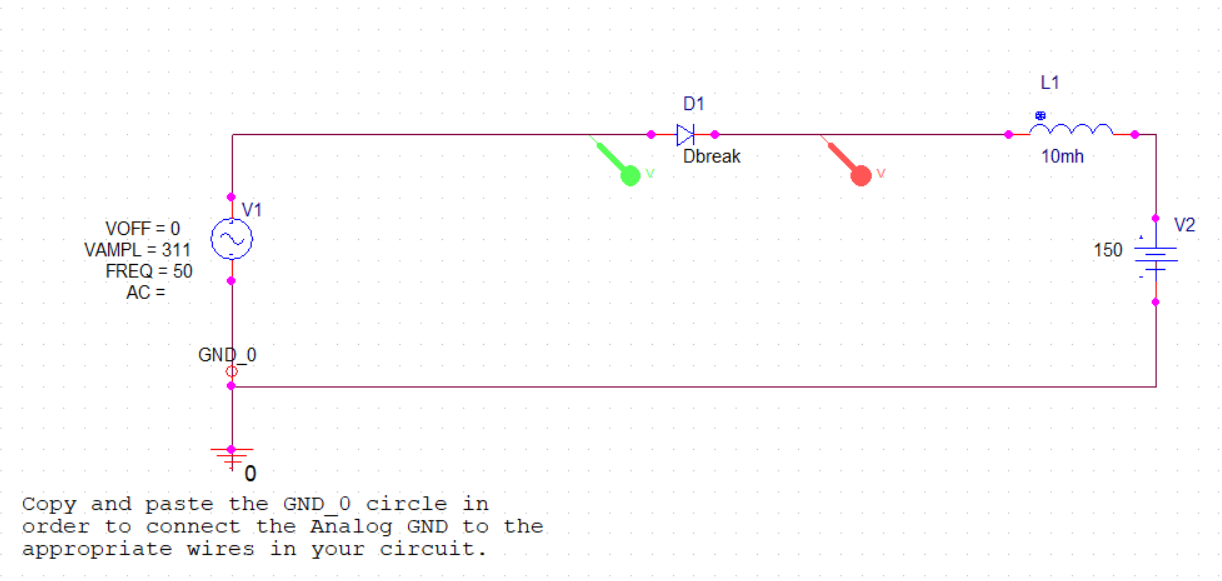
\includegraphics[scale=0.7]{Circuitos/3.png}
\caption{Diagrama Amplificador de Potencia}
\end{figure}
\newpage
\begin{figure}[hbtp]
\centering
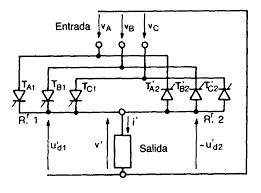
\includegraphics[scale=1]{Circuitos/4.png}
\caption{Formula Eficiencia}
\end{figure}
Dónde:
n = es la eficiencia del amplificador.\\
Pout = es la potencia de salida de los amplificadores entregada a la carga.\\
Pdc = es la potencia de CC tomada del suministro.\\
Para un amplificador de potencia, es muy importante que la fuente de alimentación de los amplificadores esté bien diseñada para proporcionar la máxima potencia continua disponible a la señal de salida.

\section*{Amplificador en una sola etapa}
\begin{figure}[hbtp]
\centering
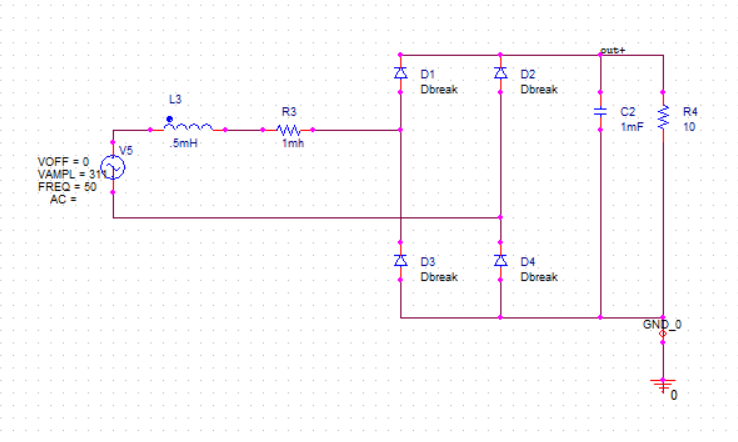
\includegraphics[scale=0.7]{Circuitos/5.png}
\caption{Circuito amplificador en una sola etapa}
\end{figure}
Este es el tipo más simple de circuito amplificador de potencia Clase A. Utiliza un transistor de extremo único para su etapa de salida con la carga resistiva conectada directamente al terminal colector. Cuando el transistor se enciende, se hunde la corriente de salida a través del Colector, lo que resulta en una caída de voltaje inevitable a través de la resistencia del Emisor, limitando así la capacidad de salida negativa.

La eficiencia de este tipo de circuito es muy baja (menos del 30 porcentaje) y ofrece pequeñas salidas de potencia para un gran drenaje en la fuente de alimentación de CC. Una etapa de amplificador de Clase A pasa la misma corriente de carga incluso cuando no se aplica señal de entrada, por lo que se necesitan disipadores de calor grandes para los transistores de salida.

\newpage
\section*{Configuraciones transistor Darlington}
\begin{figure}[hbtp]
\centering
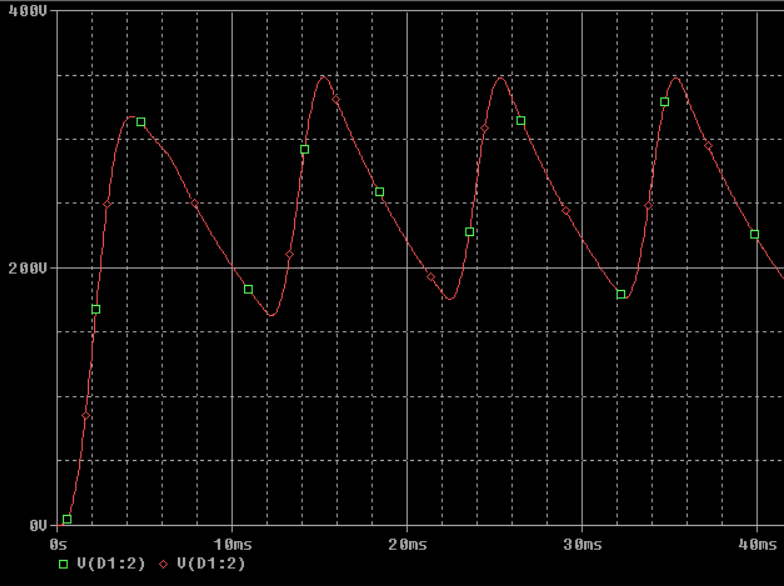
\includegraphics[scale=0.7]{Circuitos/6.png}
\caption{Circuito configuraciones transistor Darlington}
\end{figure}
La ganancia de corriente total Beta o el valor de hfe de un dispositivo Darlington es el producto de las dos ganancias individuales de los transistores multiplicadas juntas y valores de Beta muy elevados junto con altas corrientes de colector son posibles en comparación con un solo circuito de transistor.

Para mejorar la eficiencia total de potencia del amplificador de Clase A , es posible diseñar el circuito con un transformador conectado directamente en el circuito colector para formar un circuito llamado amplificador acoplado a transformador . El transformador mejora la eficiencia del amplificador al hacer coincidir la impedancia de la carga con la de la salida de los amplificadores usando la relación de vueltas ( n ) del transformador y un ejemplo de esto se da a continuación.

\section*{Amplificador acoplado a transformador}
\begin{figure}[hbtp]
\centering
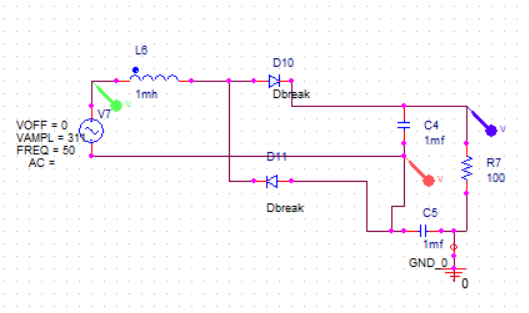
\includegraphics[scale=0.7]{Circuitos/7.png}
\caption{Circuito amplificador acoplado a transformador}
\end{figure}
\newpage
Como la corriente del colector, Ic se reduce por debajo del punto Q quieto establecido por la tensión de polarización básica, debido a las variaciones en la corriente base, el flujo magnético en el núcleo del transformador se colapsa causando una fem inducida en los devanados primarios del transformador. Esto hace que una tensión instantánea del colector aumente a un valor del doble de la tensión de alimentación de 2 Vcc, lo que da una corriente de colector máxima de dos veces Ic cuando el voltaje del colector está en su mínimo. Entonces la eficiencia de este tipo de configuración del amplificador de clase A se puede calcular de la siguiente manera.\\
\begin{figure}[hbtp]
\centering
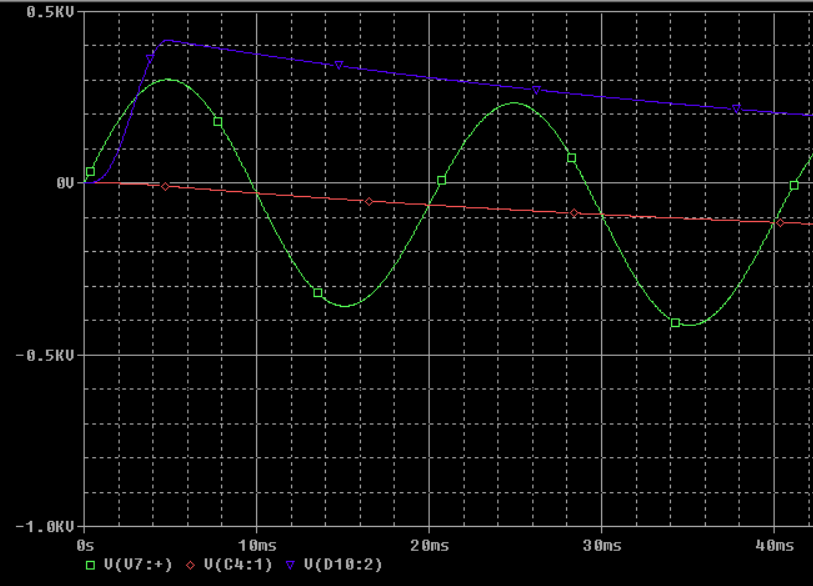
\includegraphics[scale=0.7]{Circuitos/8.png}
\caption{Formula voltaje del colector de rms}
\end{figure}

\begin{figure}[hbtp]
\centering
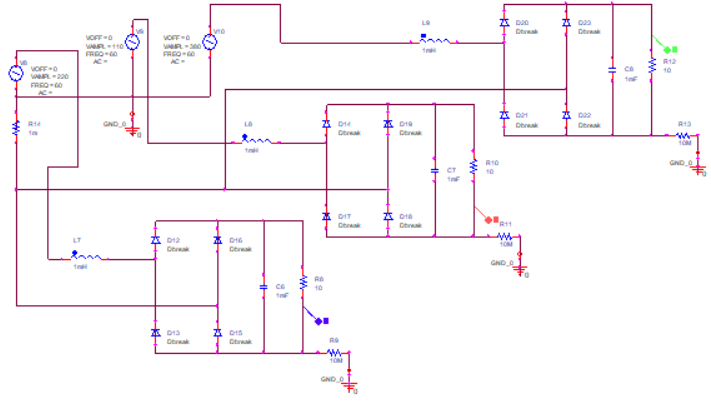
\includegraphics[scale=0.7]{Circuitos/9.png}
\caption{Formula corriente del recopilador rms}
\end{figure}

\begin{figure}[hbtp]
\centering
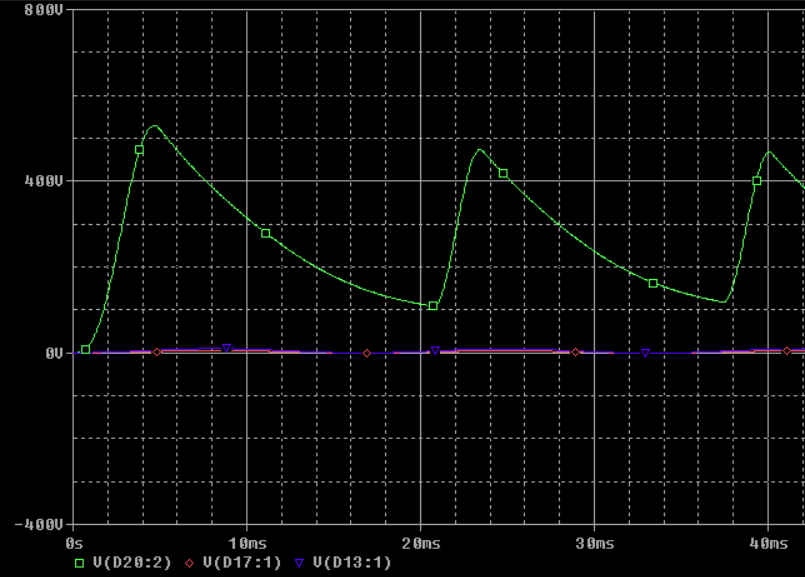
\includegraphics[scale=0.7]{Circuitos/10.png}
\caption{Formula potencia rms entregada a la carga (Pac)}
\end{figure}

\begin{figure}[hbtp]
\centering
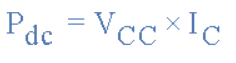
\includegraphics[scale=1]{Circuitos/11.PNG}
\caption{Formula potencia promedio extraída del suministro (Pdc)}
\end{figure}

\begin{figure}[hbtp]
\centering
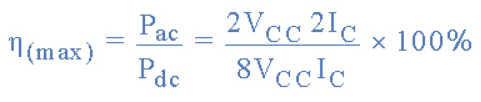
\includegraphics[scale=1]{Circuitos/12.PNG}
\caption{Formula de la eficacia de un amplificador Clase A acoplado a transformador}
\end{figure}

\newpage
Un transformador de salida mejora la eficiencia del amplificador al hacer coincidir la impedancia de la carga con la de la impedancia de salida del amplificador. 

\section{Ventaja}
La clase A se refiere a una etapa de salida con una corriente de polarización mayor que la máxima corriente de salida que dan, de tal forma que los transistores de salida siempre están consumiendo corriente. La gran ventaja de la clase A es que es casi lineal, y en consecuencia la distorsión es menor.

\section{Desventaja}
La gran desventaja de la clase A es que es poco eficiente, se requiere un amplificador de clase A muy grande para dar 50 W, y ese amplificador usa mucha corriente y se pone a muy alta temperatura.

\section*{Referencias bibliográficas}
\url{https://www.ecured.cu/Amplificador_clase_A}\\
\url{https://electronicavm.files.wordpress.com/2011/03/amplificadores-clase-a-y-b1.pdf}\\
\url{http://tutorialesdeelectronicabasica.blogspot.com/2018/06/el-amplificador-de-clase-es-un.html}

\end{document}